\documentclass[twoside]{book}

% Packages required by doxygen
\usepackage{fixltx2e}
\usepackage{calc}
\usepackage{doxygen}
\usepackage[export]{adjustbox} % also loads graphicx
\usepackage{graphicx}
\usepackage[utf8]{inputenc}
\usepackage{makeidx}
\usepackage{multicol}
\usepackage{multirow}
\PassOptionsToPackage{warn}{textcomp}
\usepackage{textcomp}
\usepackage[nointegrals]{wasysym}
\usepackage[table]{xcolor}

% Font selection
\usepackage[T1]{fontenc}
\usepackage[scaled=.90]{helvet}
\usepackage{courier}
\usepackage{amssymb}
\usepackage{sectsty}
\renewcommand{\familydefault}{\sfdefault}
\allsectionsfont{%
  \fontseries{bc}\selectfont%
  \color{darkgray}%
}
\renewcommand{\DoxyLabelFont}{%
  \fontseries{bc}\selectfont%
  \color{darkgray}%
}
\newcommand{\+}{\discretionary{\mbox{\scriptsize$\hookleftarrow$}}{}{}}

% Page & text layout
\usepackage{geometry}
\geometry{%
  a4paper,%
  top=2.5cm,%
  bottom=2.5cm,%
  left=2.5cm,%
  right=2.5cm%
}
\tolerance=750
\hfuzz=15pt
\hbadness=750
\setlength{\emergencystretch}{15pt}
\setlength{\parindent}{0cm}
\setlength{\parskip}{3ex plus 2ex minus 2ex}
\makeatletter
\renewcommand{\paragraph}{%
  \@startsection{paragraph}{4}{0ex}{-1.0ex}{1.0ex}{%
    \normalfont\normalsize\bfseries\SS@parafont%
  }%
}
\renewcommand{\subparagraph}{%
  \@startsection{subparagraph}{5}{0ex}{-1.0ex}{1.0ex}{%
    \normalfont\normalsize\bfseries\SS@subparafont%
  }%
}
\makeatother

% Headers & footers
\usepackage{fancyhdr}
\pagestyle{fancyplain}
\fancyhead[LE]{\fancyplain{}{\bfseries\thepage}}
\fancyhead[CE]{\fancyplain{}{}}
\fancyhead[RE]{\fancyplain{}{\bfseries\leftmark}}
\fancyhead[LO]{\fancyplain{}{\bfseries\rightmark}}
\fancyhead[CO]{\fancyplain{}{}}
\fancyhead[RO]{\fancyplain{}{\bfseries\thepage}}
\fancyfoot[LE]{\fancyplain{}{}}
\fancyfoot[CE]{\fancyplain{}{}}
\fancyfoot[RE]{\fancyplain{}{\bfseries\scriptsize Generated by Doxygen }}
\fancyfoot[LO]{\fancyplain{}{\bfseries\scriptsize Generated by Doxygen }}
\fancyfoot[CO]{\fancyplain{}{}}
\fancyfoot[RO]{\fancyplain{}{}}
\renewcommand{\footrulewidth}{0.4pt}
\renewcommand{\chaptermark}[1]{%
  \markboth{#1}{}%
}
\renewcommand{\sectionmark}[1]{%
  \markright{\thesection\ #1}%
}

% Indices & bibliography
\usepackage{natbib}
\usepackage[titles]{tocloft}
\setcounter{tocdepth}{3}
\setcounter{secnumdepth}{5}
\makeindex

% Hyperlinks (required, but should be loaded last)
\usepackage{ifpdf}
\ifpdf
  \usepackage[pdftex,pagebackref=true]{hyperref}
\else
  \usepackage[ps2pdf,pagebackref=true]{hyperref}
\fi
\hypersetup{%
  colorlinks=true,%
  linkcolor=blue,%
  citecolor=blue,%
  unicode%
}

% Custom commands
\newcommand{\clearemptydoublepage}{%
  \newpage{\pagestyle{empty}\cleardoublepage}%
}

\usepackage{caption}
\captionsetup{labelsep=space,justification=centering,font={bf},singlelinecheck=off,skip=4pt,position=top}

%===== C O N T E N T S =====

\begin{document}

% Titlepage & ToC
\hypersetup{pageanchor=false,
             bookmarksnumbered=true,
             pdfencoding=unicode
            }
\pagenumbering{alph}
\begin{titlepage}
\vspace*{7cm}
\begin{center}%
{\Large Proyecto Final A\+L\+SE 2020-\/1 \\[1ex]\large 0.\+1 }\\
\vspace*{1cm}
{\large Generated by Doxygen 1.8.13}\\
\end{center}
\end{titlepage}
\clearemptydoublepage
\pagenumbering{roman}
\tableofcontents
\clearemptydoublepage
\pagenumbering{arabic}
\hypersetup{pageanchor=true}

%--- Begin generated contents ---
\chapter{Hierarchical Index}
\section{Class Hierarchy}
This inheritance list is sorted roughly, but not completely, alphabetically\+:\begin{DoxyCompactList}
\item \contentsline{section}{datos\+\_\+usuario}{\pageref{classdatos__usuario}}{}
\item \contentsline{section}{D\+B\+\_\+\+Local}{\pageref{class_d_b___local}}{}
\item \contentsline{section}{prueba}{\pageref{structprueba}}{}
\item Q\+Dialog\begin{DoxyCompactList}
\item \contentsline{section}{clave\+\_\+erronea}{\pageref{classclave__erronea}}{}
\item \contentsline{section}{formulario\+\_\+paciente}{\pageref{classformulario__paciente}}{}
\item \contentsline{section}{formulario\+\_\+usuario}{\pageref{classformulario__usuario}}{}
\item \contentsline{section}{usuario}{\pageref{classusuario}}{}
\end{DoxyCompactList}
\item Q\+Main\+Window\begin{DoxyCompactList}
\item \contentsline{section}{Main\+Window}{\pageref{class_main_window}}{}
\end{DoxyCompactList}
\item \contentsline{section}{qt\+\_\+meta\+\_\+stringdata\+\_\+\+Main\+Window\+\_\+t}{\pageref{structqt__meta__stringdata___main_window__t}}{}
\item \contentsline{section}{qt\+\_\+meta\+\_\+stringdata\+\_\+usuario\+\_\+t}{\pageref{structqt__meta__stringdata__usuario__t}}{}
\item \contentsline{section}{Ui\+\_\+\+Main\+Window}{\pageref{class_ui___main_window}}{}
\begin{DoxyCompactList}
\item \contentsline{section}{Ui\+:\+:Main\+Window}{\pageref{class_ui_1_1_main_window}}{}
\end{DoxyCompactList}
\item \contentsline{section}{Ui\+\_\+usuario}{\pageref{class_ui__usuario}}{}
\begin{DoxyCompactList}
\item \contentsline{section}{Ui\+:\+:usuario}{\pageref{class_ui_1_1usuario}}{}
\end{DoxyCompactList}
\item \contentsline{section}{user\+\_\+data}{\pageref{structuser__data}}{}
\end{DoxyCompactList}

\chapter{Class Index}
\section{Class List}
Here are the classes, structs, unions and interfaces with brief descriptions\+:\begin{DoxyCompactList}
\item\contentsline{section}{\hyperlink{classclave__erronea}{clave\+\_\+erronea} \\*Se define como una ventana de dialogo, en los atributos publicos se define el constructor y destructor de la clase y en los atributos privados la ventana }{\pageref{classclave__erronea}}{}
\item\contentsline{section}{\hyperlink{classdatos__usuario}{datos\+\_\+usuario} }{\pageref{classdatos__usuario}}{}
\item\contentsline{section}{\hyperlink{class_d_b___local}{D\+B\+\_\+\+Local} \\*Se tiene en cuenta sqlite3 para la base de datos en los atributos privados se definen las funciones llamadas necesarias para comparar las contraseñas y en los atributos publicos se definen las funciones necesarias con sus parametros correspondientes }{\pageref{class_d_b___local}}{}
\item\contentsline{section}{\hyperlink{classformulario__paciente}{formulario\+\_\+paciente} \\*Se defiene como una ventana de dialogo, en los atributos publicos se define el constructor y destructor de la clase, en señales se tiene la funcion enviar\+Datos\+Pnt la cual es necesaria para enviar los datos del paciente, en los slots privados estan las funciones con sus respectivos parametros y se define el boton \char`\"{}\+O\+K\char`\"{} o \char`\"{}cancel\char`\"{} y en los atributos privados la ventana }{\pageref{classformulario__paciente}}{}
\item\contentsline{section}{\hyperlink{classformulario__usuario}{formulario\+\_\+usuario} \\*Se defiene como una ventana de dialogo en sus atributos publicos se encuentra el constructor y destructor de la clase, en signals, en esta clase se tienen dos señales una para enviar los datos del usuario nuevo y comparar y la otra para enviar los datos de un usuario nuevo, en sus slots se tienen dos opciones de ingreso uno con el boton \char`\"{}\+O\+K\char`\"{} y otro con el boton \char`\"{}registra usuario\char`\"{} y en sus atributos privados se define la clave del administrador para no dejar registrar cualquier usuario y la definicion del ui }{\pageref{classformulario__usuario}}{}
\item\contentsline{section}{\hyperlink{class_ui_1_1_main_window}{Ui\+::\+Main\+Window} }{\pageref{class_ui_1_1_main_window}}{}
\item\contentsline{section}{\hyperlink{class_main_window}{Main\+Window} \\*Es la clase mainwindow en la cual en los parametros publicos se tiene el constructor y destructor de la clase, en los slots privados se colocan las funciones de la clase con sus respectivos parametros y se definen los botones de la aplicacion y en los atributos privados se definen las variables ui, $\ast$rd, $\ast$rl, $\ast$\+\_\+timer1, $\ast$\+\_\+timer2, \+\_\+estado, estado, \+\_\+aciertos, \+\_\+errores y la base de datos }{\pageref{class_main_window}}{}
\item\contentsline{section}{\hyperlink{structprueba}{prueba} \\*The prueba struct esta estructura sirve para imprimir mas adelante la hora y si fue correcto o incorrecto cuando se oprime el boton con la aplicacion de agilidad }{\pageref{structprueba}}{}
\item\contentsline{section}{\hyperlink{structqt__meta__stringdata___main_window__t}{qt\+\_\+meta\+\_\+stringdata\+\_\+\+Main\+Window\+\_\+t} }{\pageref{structqt__meta__stringdata___main_window__t}}{}
\item\contentsline{section}{\hyperlink{structqt__meta__stringdata__usuario__t}{qt\+\_\+meta\+\_\+stringdata\+\_\+usuario\+\_\+t} }{\pageref{structqt__meta__stringdata__usuario__t}}{}
\item\contentsline{section}{\hyperlink{class_ui___main_window}{Ui\+\_\+\+Main\+Window} }{\pageref{class_ui___main_window}}{}
\item\contentsline{section}{\hyperlink{class_ui__usuario}{Ui\+\_\+usuario} }{\pageref{class_ui__usuario}}{}
\item\contentsline{section}{\hyperlink{structuser__data}{user\+\_\+data} }{\pageref{structuser__data}}{}
\item\contentsline{section}{\hyperlink{class_ui_1_1usuario}{Ui\+::usuario} }{\pageref{class_ui_1_1usuario}}{}
\item\contentsline{section}{\hyperlink{classusuario}{usuario} }{\pageref{classusuario}}{}
\end{DoxyCompactList}

\chapter{Class Documentation}
\hypertarget{classclave__erronea}{}\section{clave\+\_\+erronea Class Reference}
\label{classclave__erronea}\index{clave\+\_\+erronea@{clave\+\_\+erronea}}


The \hyperlink{classclave__erronea}{clave\+\_\+erronea} class se define como una ventana de dialogo, en los atributos publicos se define el constructor y destructor de la clase y en los atributos privados la ventana.  




{\ttfamily \#include $<$clave\+\_\+erronea.\+h$>$}

Inheritance diagram for clave\+\_\+erronea\+:\begin{figure}[H]
\begin{center}
\leavevmode
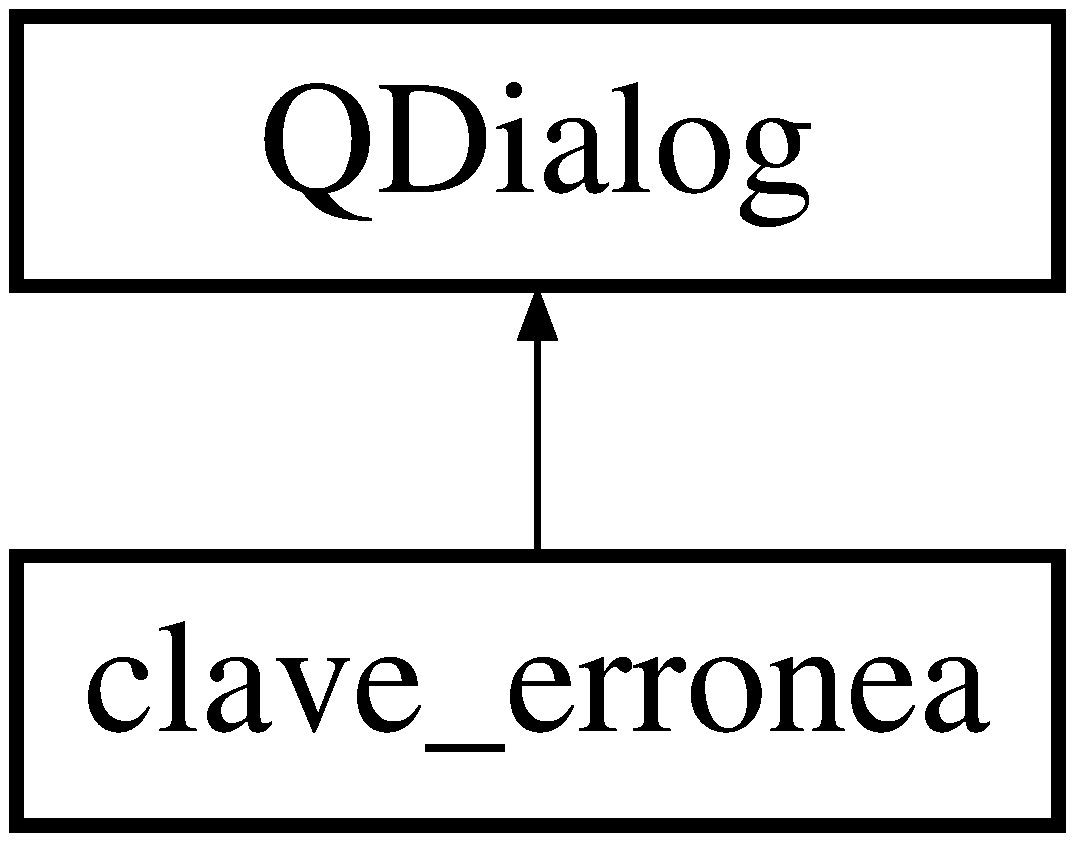
\includegraphics[height=2.000000cm]{classclave__erronea}
\end{center}
\end{figure}
\subsection*{Public Member Functions}
\begin{DoxyCompactItemize}
\item 
\hyperlink{classclave__erronea_ac304b7fa422028fb2f4a63a0b18da520}{clave\+\_\+erronea} (Q\+Widget $\ast$parent=0)
\begin{DoxyCompactList}\small\item\em \hyperlink{classclave__erronea_ac304b7fa422028fb2f4a63a0b18da520}{clave\+\_\+erronea\+::clave\+\_\+erronea} es una ventana de dialogo la cual va a aparecer si el usuario o la contraseña son incorrectos o cuando la clave del administrador para ingresar un usuario nuevo es incorrecta a la guardada por el sistema \end{DoxyCompactList}\item 
\mbox{\Hypertarget{classclave__erronea_a0c445695b22b66d7a4e24bad293cf5df}\label{classclave__erronea_a0c445695b22b66d7a4e24bad293cf5df}} 
\hyperlink{classclave__erronea_a0c445695b22b66d7a4e24bad293cf5df}{$\sim$clave\+\_\+erronea} ()
\begin{DoxyCompactList}\small\item\em \hyperlink{classclave__erronea_a0c445695b22b66d7a4e24bad293cf5df}{clave\+\_\+erronea\+::$\sim$clave\+\_\+erronea} es el destructor de la clase \end{DoxyCompactList}\end{DoxyCompactItemize}


\subsection{Detailed Description}
The \hyperlink{classclave__erronea}{clave\+\_\+erronea} class se define como una ventana de dialogo, en los atributos publicos se define el constructor y destructor de la clase y en los atributos privados la ventana. 

\subsection{Constructor \& Destructor Documentation}
\mbox{\Hypertarget{classclave__erronea_ac304b7fa422028fb2f4a63a0b18da520}\label{classclave__erronea_ac304b7fa422028fb2f4a63a0b18da520}} 
\index{clave\+\_\+erronea@{clave\+\_\+erronea}!clave\+\_\+erronea@{clave\+\_\+erronea}}
\index{clave\+\_\+erronea@{clave\+\_\+erronea}!clave\+\_\+erronea@{clave\+\_\+erronea}}
\subsubsection{\texorpdfstring{clave\+\_\+erronea()}{clave\_erronea()}}
{\footnotesize\ttfamily clave\+\_\+erronea\+::clave\+\_\+erronea (\begin{DoxyParamCaption}\item[{Q\+Widget $\ast$}]{parent = {\ttfamily 0} }\end{DoxyParamCaption})\hspace{0.3cm}{\ttfamily [explicit]}}



\hyperlink{classclave__erronea_ac304b7fa422028fb2f4a63a0b18da520}{clave\+\_\+erronea\+::clave\+\_\+erronea} es una ventana de dialogo la cual va a aparecer si el usuario o la contraseña son incorrectos o cuando la clave del administrador para ingresar un usuario nuevo es incorrecta a la guardada por el sistema 


\begin{DoxyParams}{Parameters}
{\em parent} & \\
\hline
\end{DoxyParams}


The documentation for this class was generated from the following files\+:\begin{DoxyCompactItemize}
\item 
/home/alseuser/\+Proyecto\+A\+L\+S\+E/clave\+\_\+erronea.\+h\item 
/home/alseuser/\+Proyecto\+A\+L\+S\+E/clave\+\_\+erronea.\+cpp\end{DoxyCompactItemize}

\hypertarget{classdatos__usuario}{}\section{datos\+\_\+usuario Class Reference}
\label{classdatos__usuario}\index{datos\+\_\+usuario@{datos\+\_\+usuario}}
\subsection*{Public Member Functions}
\begin{DoxyCompactItemize}
\item 
\mbox{\Hypertarget{classdatos__usuario_aa63024d7b03ba8bd08748a29b9ee436a}\label{classdatos__usuario_aa63024d7b03ba8bd08748a29b9ee436a}} 
void {\bfseries set\+Usr\+Data} (\hyperlink{structuser__data}{user\+\_\+data} Usr\+Data)
\item 
\mbox{\Hypertarget{classdatos__usuario_a4c580e077e65cdaa6057e92c15ccec60}\label{classdatos__usuario_a4c580e077e65cdaa6057e92c15ccec60}} 
\hyperlink{structuser__data}{user\+\_\+data} {\bfseries get\+Usr\+Data} ()
\item 
\mbox{\Hypertarget{classdatos__usuario_a931103dd6b8abceb0497136df21ca24c}\label{classdatos__usuario_a931103dd6b8abceb0497136df21ca24c}} 
{\bfseries datos\+\_\+usuario} (\hyperlink{structuser__data}{user\+\_\+data} datos)
\end{DoxyCompactItemize}


The documentation for this class was generated from the following files\+:\begin{DoxyCompactItemize}
\item 
/home/alseuser/\+Proyecto\+A\+L\+S\+E/datos\+\_\+usuario.\+h\item 
/home/alseuser/\+Proyecto\+A\+L\+S\+E/datos\+\_\+usuario.\+cpp\item 
/home/alseuser/\+Proyecto\+A\+L\+S\+E/datos\+\_\+usuario\+\_\+copy.\+cpp\end{DoxyCompactItemize}

\hypertarget{class_d_b___local}{}\section{D\+B\+\_\+\+Local Class Reference}
\label{class_d_b___local}\index{D\+B\+\_\+\+Local@{D\+B\+\_\+\+Local}}


The \hyperlink{class_d_b___local}{D\+B\+\_\+\+Local} class se tiene en cuenta sqlite3 para la base de datos en los atributos privados se definen las funciones llamadas necesarias para comparar las contraseñas y en los atributos publicos se definen las funciones necesarias con sus parametros correspondientes.  




{\ttfamily \#include $<$db\+\_\+local.\+h$>$}

\subsection*{Public Member Functions}
\begin{DoxyCompactItemize}
\item 
\mbox{\Hypertarget{class_d_b___local_a439c348ad67f06527f46ee2ddbfbcb05}\label{class_d_b___local_a439c348ad67f06527f46ee2ddbfbcb05}} 
\hyperlink{class_d_b___local_a439c348ad67f06527f46ee2ddbfbcb05}{D\+B\+\_\+\+Local} ()
\begin{DoxyCompactList}\small\item\em \hyperlink{class_d_b___local_a439c348ad67f06527f46ee2ddbfbcb05}{D\+B\+\_\+\+Local\+::\+D\+B\+\_\+\+Local} es el constructor de la clase. \end{DoxyCompactList}\item 
bool \hyperlink{class_d_b___local_af177cdf53157cb7da307a50b95b19001}{almacenar\+Paciente} (string Nombre, string apellido, int edad, int documento, string genero, string raza, string ingresos)
\begin{DoxyCompactList}\small\item\em \hyperlink{class_d_b___local_af177cdf53157cb7da307a50b95b19001}{D\+B\+\_\+\+Local\+::almacenar\+Paciente} con esta funcion se guarda los datos del paciente en la base de datos respectiva. \end{DoxyCompactList}\item 
bool \hyperlink{class_d_b___local_ad8637aa272a8a361ae2a6e1e7f8cd71c}{abrir\+DB} (string path)
\begin{DoxyCompactList}\small\item\em \hyperlink{class_d_b___local_ad8637aa272a8a361ae2a6e1e7f8cd71c}{D\+B\+\_\+\+Local\+::abrir\+DB} abre la base de datos. \end{DoxyCompactList}\item 
int \hyperlink{class_d_b___local_a7812291d7772ef9b4a4e4bfe0cac3a09}{comparar\+Datos\+Usuario} (string nombre\+Usuario, string contrasena)
\begin{DoxyCompactList}\small\item\em \hyperlink{class_d_b___local_a7812291d7772ef9b4a4e4bfe0cac3a09}{D\+B\+\_\+\+Local\+::comparar\+Datos\+Usuario} esta funcion se le pasan los nombres de usuario y la contraseña que se ingreso si el usuario ya esta registrado para comparar que estos datos esten en la base de datos. \end{DoxyCompactList}\item 
bool \hyperlink{class_d_b___local_a021938e1e159fd8c2f6876f2a74d6655}{almacenar\+Usuario} (string nombre\+Usuario, string password, string Nombre, string apellido, int documento, int edad)
\begin{DoxyCompactList}\small\item\em \hyperlink{class_d_b___local_a021938e1e159fd8c2f6876f2a74d6655}{D\+B\+\_\+\+Local\+::almacenar\+Usuario} con esta funcion se guarda los datos del usuario nuevo en la base de datos. \end{DoxyCompactList}\item 
bool \hyperlink{class_d_b___local_aa5f3f6315c55e86a030da1c4c9b3a4cb}{cerrar\+DB} ()
\begin{DoxyCompactList}\small\item\em \hyperlink{class_d_b___local_aa5f3f6315c55e86a030da1c4c9b3a4cb}{D\+B\+\_\+\+Local\+::cerrar\+DB} esta funcion cierra la base de datos. \end{DoxyCompactList}\end{DoxyCompactItemize}


\subsection{Detailed Description}
The \hyperlink{class_d_b___local}{D\+B\+\_\+\+Local} class se tiene en cuenta sqlite3 para la base de datos en los atributos privados se definen las funciones llamadas necesarias para comparar las contraseñas y en los atributos publicos se definen las funciones necesarias con sus parametros correspondientes. 

\subsection{Member Function Documentation}
\mbox{\Hypertarget{class_d_b___local_ad8637aa272a8a361ae2a6e1e7f8cd71c}\label{class_d_b___local_ad8637aa272a8a361ae2a6e1e7f8cd71c}} 
\index{D\+B\+\_\+\+Local@{D\+B\+\_\+\+Local}!abrir\+DB@{abrir\+DB}}
\index{abrir\+DB@{abrir\+DB}!D\+B\+\_\+\+Local@{D\+B\+\_\+\+Local}}
\subsubsection{\texorpdfstring{abrir\+D\+B()}{abrirDB()}}
{\footnotesize\ttfamily bool D\+B\+\_\+\+Local\+::abrir\+DB (\begin{DoxyParamCaption}\item[{string}]{path }\end{DoxyParamCaption})}



\hyperlink{class_d_b___local_ad8637aa272a8a361ae2a6e1e7f8cd71c}{D\+B\+\_\+\+Local\+::abrir\+DB} abre la base de datos. 


\begin{DoxyParams}{Parameters}
{\em path} & es el archivo de la base de datos \\
\hline
\end{DoxyParams}
\begin{DoxyReturn}{Returns}
true si puede abrir la base de datos o false si no puede abrir la base de datos y un mensaje en la pantalla 
\end{DoxyReturn}
abre la base de datos\mbox{\Hypertarget{class_d_b___local_af177cdf53157cb7da307a50b95b19001}\label{class_d_b___local_af177cdf53157cb7da307a50b95b19001}} 
\index{D\+B\+\_\+\+Local@{D\+B\+\_\+\+Local}!almacenar\+Paciente@{almacenar\+Paciente}}
\index{almacenar\+Paciente@{almacenar\+Paciente}!D\+B\+\_\+\+Local@{D\+B\+\_\+\+Local}}
\subsubsection{\texorpdfstring{almacenar\+Paciente()}{almacenarPaciente()}}
{\footnotesize\ttfamily bool D\+B\+\_\+\+Local\+::almacenar\+Paciente (\begin{DoxyParamCaption}\item[{string}]{Nombre,  }\item[{string}]{apellido,  }\item[{int}]{edad,  }\item[{int}]{documento,  }\item[{string}]{ingresos,  }\item[{string}]{genero,  }\item[{string}]{raza }\end{DoxyParamCaption})}



\hyperlink{class_d_b___local_af177cdf53157cb7da307a50b95b19001}{D\+B\+\_\+\+Local\+::almacenar\+Paciente} con esta funcion se guarda los datos del paciente en la base de datos respectiva. 


\begin{DoxyParams}{Parameters}
{\em Nombre} & nombre del paciente \\
\hline
{\em apellido} & apellido del paciente \\
\hline
{\em edad} & edad del paciente \\
\hline
{\em documento} & documento del paciente \\
\hline
{\em ingresos} & nivel de ingresos del paciente \\
\hline
{\em genero} & genero del paciente \\
\hline
{\em raza} & raza del paciente \\
\hline
\end{DoxyParams}
\begin{DoxyReturn}{Returns}
true si puede guardar correctamente los datos del paciente en la base de datos o false si no puede guardar la informacion 
\end{DoxyReturn}
\mbox{\Hypertarget{class_d_b___local_a021938e1e159fd8c2f6876f2a74d6655}\label{class_d_b___local_a021938e1e159fd8c2f6876f2a74d6655}} 
\index{D\+B\+\_\+\+Local@{D\+B\+\_\+\+Local}!almacenar\+Usuario@{almacenar\+Usuario}}
\index{almacenar\+Usuario@{almacenar\+Usuario}!D\+B\+\_\+\+Local@{D\+B\+\_\+\+Local}}
\subsubsection{\texorpdfstring{almacenar\+Usuario()}{almacenarUsuario()}}
{\footnotesize\ttfamily bool D\+B\+\_\+\+Local\+::almacenar\+Usuario (\begin{DoxyParamCaption}\item[{string}]{nombre\+Usuario,  }\item[{string}]{password,  }\item[{string}]{Nombre,  }\item[{string}]{apellido,  }\item[{int}]{documento,  }\item[{int}]{edad }\end{DoxyParamCaption})}



\hyperlink{class_d_b___local_a021938e1e159fd8c2f6876f2a74d6655}{D\+B\+\_\+\+Local\+::almacenar\+Usuario} con esta funcion se guarda los datos del usuario nuevo en la base de datos. 


\begin{DoxyParams}{Parameters}
{\em nombre\+Usuario} & el nombre con el cual el usuario va a poder iniciar sesion \\
\hline
{\em password} & la clave del usuario \\
\hline
{\em Nombre} & nombre del usuario \\
\hline
{\em apellido} & apellido del usuario \\
\hline
{\em documento} & documento del paciente \\
\hline
{\em edad} & edad del paciente \\
\hline
\end{DoxyParams}
\begin{DoxyReturn}{Returns}
true si puede almacenar correctamente los datos y false si no puede almacenar los datos 
\end{DoxyReturn}
\mbox{\Hypertarget{class_d_b___local_aa5f3f6315c55e86a030da1c4c9b3a4cb}\label{class_d_b___local_aa5f3f6315c55e86a030da1c4c9b3a4cb}} 
\index{D\+B\+\_\+\+Local@{D\+B\+\_\+\+Local}!cerrar\+DB@{cerrar\+DB}}
\index{cerrar\+DB@{cerrar\+DB}!D\+B\+\_\+\+Local@{D\+B\+\_\+\+Local}}
\subsubsection{\texorpdfstring{cerrar\+D\+B()}{cerrarDB()}}
{\footnotesize\ttfamily bool D\+B\+\_\+\+Local\+::cerrar\+DB (\begin{DoxyParamCaption}{ }\end{DoxyParamCaption})}



\hyperlink{class_d_b___local_aa5f3f6315c55e86a030da1c4c9b3a4cb}{D\+B\+\_\+\+Local\+::cerrar\+DB} esta funcion cierra la base de datos. 

\begin{DoxyReturn}{Returns}

\end{DoxyReturn}
\mbox{\Hypertarget{class_d_b___local_a7812291d7772ef9b4a4e4bfe0cac3a09}\label{class_d_b___local_a7812291d7772ef9b4a4e4bfe0cac3a09}} 
\index{D\+B\+\_\+\+Local@{D\+B\+\_\+\+Local}!comparar\+Datos\+Usuario@{comparar\+Datos\+Usuario}}
\index{comparar\+Datos\+Usuario@{comparar\+Datos\+Usuario}!D\+B\+\_\+\+Local@{D\+B\+\_\+\+Local}}
\subsubsection{\texorpdfstring{comparar\+Datos\+Usuario()}{compararDatosUsuario()}}
{\footnotesize\ttfamily int D\+B\+\_\+\+Local\+::comparar\+Datos\+Usuario (\begin{DoxyParamCaption}\item[{string}]{nombre\+Usuario,  }\item[{string}]{contrasena }\end{DoxyParamCaption})}



\hyperlink{class_d_b___local_a7812291d7772ef9b4a4e4bfe0cac3a09}{D\+B\+\_\+\+Local\+::comparar\+Datos\+Usuario} esta funcion se le pasan los nombres de usuario y la contraseña que se ingreso si el usuario ya esta registrado para comparar que estos datos esten en la base de datos. 


\begin{DoxyParams}{Parameters}
{\em nombre\+Usuario} & nombre de usuario ingresado por el usuario para comparar que este en la base de datos \\
\hline
{\em contrasena} & contraseña del usuario despues de verificar que este el nombre de usuario en la base de datos se llama la funcion llamada u para comparar las contraseñas \\
\hline
\end{DoxyParams}
\begin{DoxyReturn}{Returns}
1 si el nombre de usuario no esta bien 2 si la contraseña es incorrecta y 0 si los datos son correctos 
\end{DoxyReturn}


The documentation for this class was generated from the following files\+:\begin{DoxyCompactItemize}
\item 
/home/alseuser/\+Proyecto\+A\+L\+S\+E/db\+\_\+local.\+h\item 
/home/alseuser/\+Proyecto\+A\+L\+S\+E/db\+\_\+local.\+cpp\end{DoxyCompactItemize}

\hypertarget{classformulario__paciente}{}\section{formulario\+\_\+paciente Class Reference}
\label{classformulario__paciente}\index{formulario\+\_\+paciente@{formulario\+\_\+paciente}}


The \hyperlink{classformulario__paciente}{formulario\+\_\+paciente} class se defiene como una ventana de dialogo, en los atributos publicos se define el constructor y destructor de la clase, en señales se tiene la funcion enviar\+Datos\+Pnt la cual es necesaria para enviar los datos del paciente, en los slots privados estan las funciones con sus respectivos parametros y se define el boton \char`\"{}\+O\+K\char`\"{} o \char`\"{}cancel\char`\"{} y en los atributos privados la ventana.  




{\ttfamily \#include $<$formulario\+\_\+paciente.\+h$>$}

Inheritance diagram for formulario\+\_\+paciente\+:\begin{figure}[H]
\begin{center}
\leavevmode
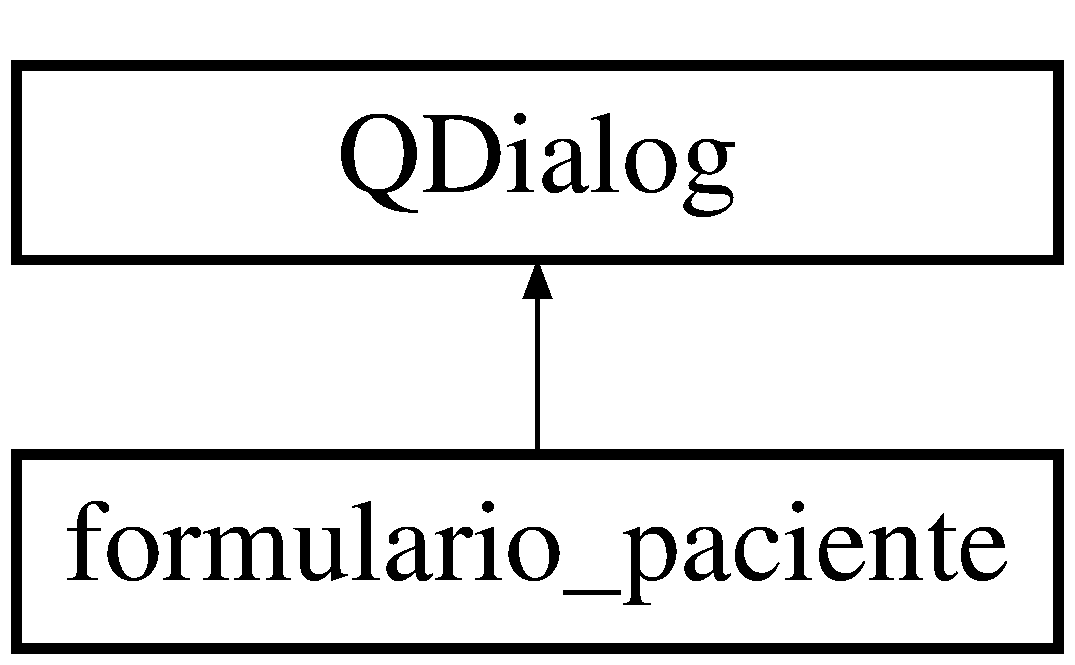
\includegraphics[height=2.000000cm]{classformulario__paciente}
\end{center}
\end{figure}
\subsection*{Signals}
\begin{DoxyCompactItemize}
\item 
\mbox{\Hypertarget{classformulario__paciente_a40f4ae3f9eda97e8b57609c0a91e1184}\label{classformulario__paciente_a40f4ae3f9eda97e8b57609c0a91e1184}} 
void {\bfseries enviar\+Datos\+Pnt} (string nombre\+Pnt, string apellido\+Pnt, int edad, long doc\+Pnt, string genero\+Pnt, string raza\+Pnt, string nivel\+S\+Epnt, bool aceptado)
\end{DoxyCompactItemize}
\subsection*{Public Member Functions}
\begin{DoxyCompactItemize}
\item 
\hyperlink{classformulario__paciente_ad200fdaad0f9dca8f1b55831d8fee231}{formulario\+\_\+paciente} (Q\+Widget $\ast$parent=0)
\begin{DoxyCompactList}\small\item\em \hyperlink{classformulario__paciente_ad200fdaad0f9dca8f1b55831d8fee231}{formulario\+\_\+paciente\+::formulario\+\_\+paciente} es el constructor de la clase \end{DoxyCompactList}\item 
\mbox{\Hypertarget{classformulario__paciente_a2cd63626c086806c4040c440322eae47}\label{classformulario__paciente_a2cd63626c086806c4040c440322eae47}} 
\hyperlink{classformulario__paciente_a2cd63626c086806c4040c440322eae47}{$\sim$formulario\+\_\+paciente} ()
\begin{DoxyCompactList}\small\item\em \hyperlink{classformulario__paciente_a2cd63626c086806c4040c440322eae47}{formulario\+\_\+paciente\+::$\sim$formulario\+\_\+paciente} es el destructor de la clase \end{DoxyCompactList}\end{DoxyCompactItemize}


\subsection{Detailed Description}
The \hyperlink{classformulario__paciente}{formulario\+\_\+paciente} class se defiene como una ventana de dialogo, en los atributos publicos se define el constructor y destructor de la clase, en señales se tiene la funcion enviar\+Datos\+Pnt la cual es necesaria para enviar los datos del paciente, en los slots privados estan las funciones con sus respectivos parametros y se define el boton \char`\"{}\+O\+K\char`\"{} o \char`\"{}cancel\char`\"{} y en los atributos privados la ventana. 

\subsection{Constructor \& Destructor Documentation}
\mbox{\Hypertarget{classformulario__paciente_ad200fdaad0f9dca8f1b55831d8fee231}\label{classformulario__paciente_ad200fdaad0f9dca8f1b55831d8fee231}} 
\index{formulario\+\_\+paciente@{formulario\+\_\+paciente}!formulario\+\_\+paciente@{formulario\+\_\+paciente}}
\index{formulario\+\_\+paciente@{formulario\+\_\+paciente}!formulario\+\_\+paciente@{formulario\+\_\+paciente}}
\subsubsection{\texorpdfstring{formulario\+\_\+paciente()}{formulario\_paciente()}}
{\footnotesize\ttfamily formulario\+\_\+paciente\+::formulario\+\_\+paciente (\begin{DoxyParamCaption}\item[{Q\+Widget $\ast$}]{parent = {\ttfamily 0} }\end{DoxyParamCaption})\hspace{0.3cm}{\ttfamily [explicit]}}



\hyperlink{classformulario__paciente_ad200fdaad0f9dca8f1b55831d8fee231}{formulario\+\_\+paciente\+::formulario\+\_\+paciente} es el constructor de la clase 


\begin{DoxyParams}{Parameters}
{\em parent} & es una ventana de dialogo la cual se va a habilitar desde el mainwindow con el boton de registro \\
\hline
\end{DoxyParams}


The documentation for this class was generated from the following files\+:\begin{DoxyCompactItemize}
\item 
/home/alseuser/\+Proyecto\+A\+L\+S\+E/formulario\+\_\+paciente.\+h\item 
/home/alseuser/\+Proyecto\+A\+L\+S\+E/formulario\+\_\+paciente.\+cpp\end{DoxyCompactItemize}

\hypertarget{classformulario__usuario}{}\section{formulario\+\_\+usuario Class Reference}
\label{classformulario__usuario}\index{formulario\+\_\+usuario@{formulario\+\_\+usuario}}


The \hyperlink{classformulario__usuario}{formulario\+\_\+usuario} class se defiene como una ventana de dialogo en sus atributos publicos se encuentra el constructor y destructor de la clase, en signals, en esta clase se tienen dos señales una para enviar los datos del usuario nuevo y comparar y la otra para enviar los datos de un usuario nuevo, en sus slots se tienen dos opciones de ingreso uno con el boton \char`\"{}\+O\+K\char`\"{} y otro con el boton \char`\"{}registra usuario\char`\"{} y en sus atributos privados se define la clave del administrador para no dejar registrar cualquier usuario y la definicion del ui.  




{\ttfamily \#include $<$formulario\+\_\+usuario.\+h$>$}

Inheritance diagram for formulario\+\_\+usuario\+:\begin{figure}[H]
\begin{center}
\leavevmode
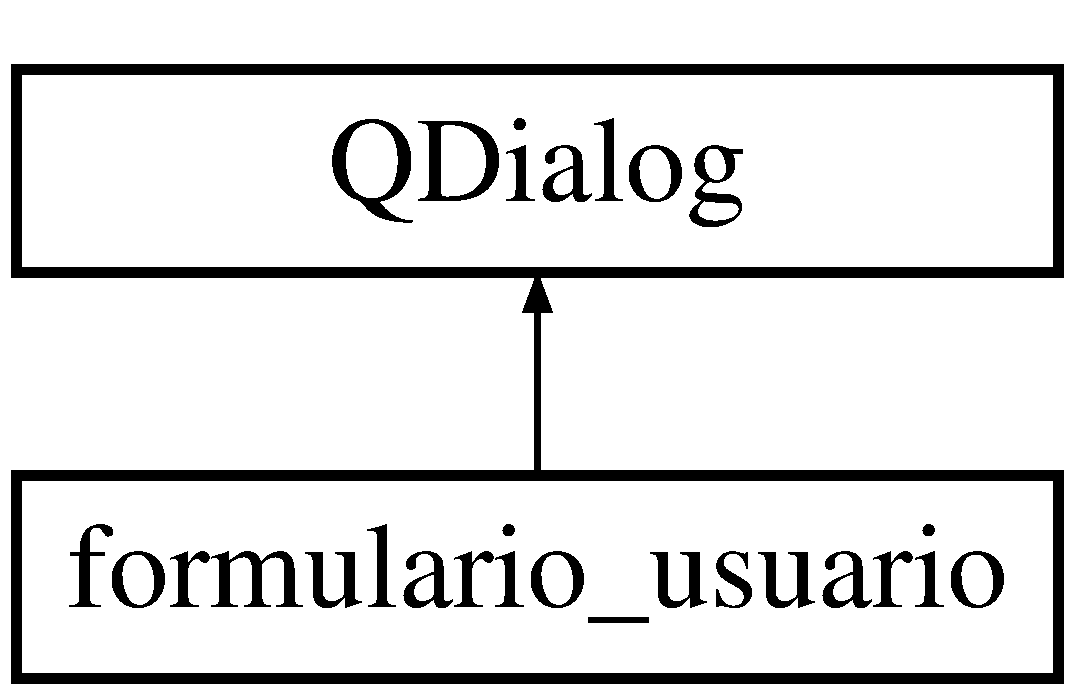
\includegraphics[height=2.000000cm]{classformulario__usuario}
\end{center}
\end{figure}
\subsection*{Signals}
\begin{DoxyCompactItemize}
\item 
\mbox{\Hypertarget{classformulario__usuario_a97c1cd74da8cc98b6ba4eb8cc6d0c5e1}\label{classformulario__usuario_a97c1cd74da8cc98b6ba4eb8cc6d0c5e1}} 
void {\bfseries enviar\+Datos} (string username, string usrpassword)
\item 
\mbox{\Hypertarget{classformulario__usuario_a9625df01df8528888cfff9e0b7a3ce5f}\label{classformulario__usuario_a9625df01df8528888cfff9e0b7a3ce5f}} 
void {\bfseries envio\+Datos\+Usuario\+New} (string usernameN, string nameN, string apellidoN, string passwordN, int doc\+IdN, int day\+NR, int month\+NR, int year\+NR, bool aceptado\+Us)
\end{DoxyCompactItemize}
\subsection*{Public Member Functions}
\begin{DoxyCompactItemize}
\item 
\hyperlink{classformulario__usuario_a85cf7bd7b98128c1690d7825b0d6493d}{formulario\+\_\+usuario} (Q\+Widget $\ast$parent=0)
\begin{DoxyCompactList}\small\item\em \hyperlink{classformulario__usuario_a85cf7bd7b98128c1690d7825b0d6493d}{formulario\+\_\+usuario\+::formulario\+\_\+usuario} es el constructor de la clase \end{DoxyCompactList}\item 
\mbox{\Hypertarget{classformulario__usuario_a5e4007c79bdb22b028d339b0c9fae3f1}\label{classformulario__usuario_a5e4007c79bdb22b028d339b0c9fae3f1}} 
\hyperlink{classformulario__usuario_a5e4007c79bdb22b028d339b0c9fae3f1}{$\sim$formulario\+\_\+usuario} ()
\begin{DoxyCompactList}\small\item\em \hyperlink{classformulario__usuario_a5e4007c79bdb22b028d339b0c9fae3f1}{formulario\+\_\+usuario\+::$\sim$formulario\+\_\+usuario} es el destructor de la clase \end{DoxyCompactList}\end{DoxyCompactItemize}


\subsection{Detailed Description}
The \hyperlink{classformulario__usuario}{formulario\+\_\+usuario} class se defiene como una ventana de dialogo en sus atributos publicos se encuentra el constructor y destructor de la clase, en signals, en esta clase se tienen dos señales una para enviar los datos del usuario nuevo y comparar y la otra para enviar los datos de un usuario nuevo, en sus slots se tienen dos opciones de ingreso uno con el boton \char`\"{}\+O\+K\char`\"{} y otro con el boton \char`\"{}registra usuario\char`\"{} y en sus atributos privados se define la clave del administrador para no dejar registrar cualquier usuario y la definicion del ui. 

\subsection{Constructor \& Destructor Documentation}
\mbox{\Hypertarget{classformulario__usuario_a85cf7bd7b98128c1690d7825b0d6493d}\label{classformulario__usuario_a85cf7bd7b98128c1690d7825b0d6493d}} 
\index{formulario\+\_\+usuario@{formulario\+\_\+usuario}!formulario\+\_\+usuario@{formulario\+\_\+usuario}}
\index{formulario\+\_\+usuario@{formulario\+\_\+usuario}!formulario\+\_\+usuario@{formulario\+\_\+usuario}}
\subsubsection{\texorpdfstring{formulario\+\_\+usuario()}{formulario\_usuario()}}
{\footnotesize\ttfamily formulario\+\_\+usuario\+::formulario\+\_\+usuario (\begin{DoxyParamCaption}\item[{Q\+Widget $\ast$}]{parent = {\ttfamily 0} }\end{DoxyParamCaption})\hspace{0.3cm}{\ttfamily [explicit]}}



\hyperlink{classformulario__usuario_a85cf7bd7b98128c1690d7825b0d6493d}{formulario\+\_\+usuario\+::formulario\+\_\+usuario} es el constructor de la clase 


\begin{DoxyParams}{Parameters}
{\em parent} & es una ventana de dialogo la cual se va a habilitar desde el mainwindow con el boton de ingreso \\
\hline
\end{DoxyParams}


The documentation for this class was generated from the following files\+:\begin{DoxyCompactItemize}
\item 
/home/alseuser/\+Proyecto\+A\+L\+S\+E/formulario\+\_\+usuario.\+h\item 
/home/alseuser/\+Proyecto\+A\+L\+S\+E/formulario\+\_\+usuario.\+cpp\end{DoxyCompactItemize}

\hypertarget{class_ui_1_1_main_window}{}\section{Ui\+:\+:Main\+Window Class Reference}
\label{class_ui_1_1_main_window}\index{Ui\+::\+Main\+Window@{Ui\+::\+Main\+Window}}
Inheritance diagram for Ui\+:\+:Main\+Window\+:\begin{figure}[H]
\begin{center}
\leavevmode
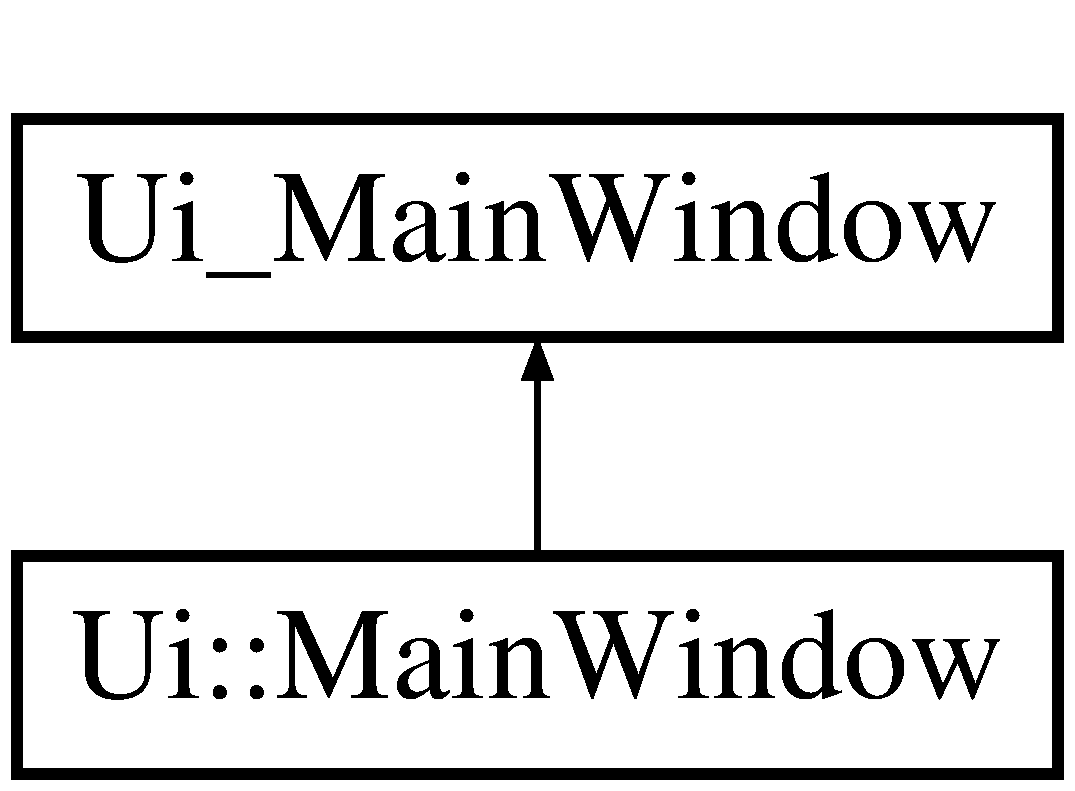
\includegraphics[height=2.000000cm]{class_ui_1_1_main_window}
\end{center}
\end{figure}
\subsection*{Additional Inherited Members}


The documentation for this class was generated from the following file\+:\begin{DoxyCompactItemize}
\item 
/home/alseuser/\+Proyecto\+A\+L\+S\+E/build-\/\+Proyecto\+A\+L\+S\+E-\/\+Desktop-\/\+Debug/ui\+\_\+mainwindow.\+h\end{DoxyCompactItemize}

\hypertarget{class_main_window}{}\section{Main\+Window Class Reference}
\label{class_main_window}\index{Main\+Window@{Main\+Window}}


The \hyperlink{class_main_window}{Main\+Window} class es la clase mainwindow en la cual en los parametros publicos se tiene el constructor y destructor de la clase, en los slots privados se colocan las funciones de la clase con sus respectivos parametros y se definen los botones de la aplicacion y en los atributos privados se definen las variables ui, $\ast$rd, $\ast$rl, $\ast$\+\_\+timer1, $\ast$\+\_\+timer2, \+\_\+estado, estado, \+\_\+aciertos, \+\_\+errores y la base de datos.  




{\ttfamily \#include $<$mainwindow.\+h$>$}

Inheritance diagram for Main\+Window\+:\begin{figure}[H]
\begin{center}
\leavevmode
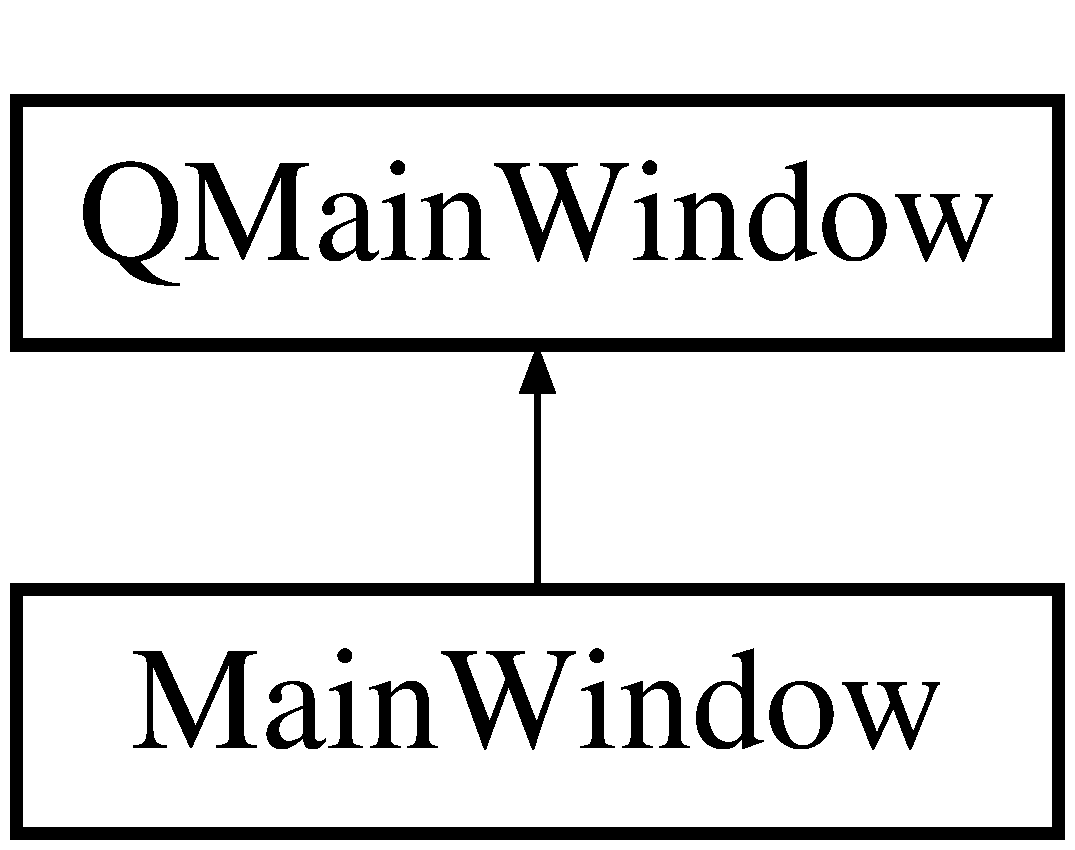
\includegraphics[height=2.000000cm]{class_main_window}
\end{center}
\end{figure}
\subsection*{Public Member Functions}
\begin{DoxyCompactItemize}
\item 
\hyperlink{class_main_window_a8b244be8b7b7db1b08de2a2acb9409db}{Main\+Window} (Q\+Widget $\ast$parent=0)
\begin{DoxyCompactList}\small\item\em \hyperlink{class_main_window_a8b244be8b7b7db1b08de2a2acb9409db}{Main\+Window\+::\+Main\+Window}. \end{DoxyCompactList}\item 
\hyperlink{class_main_window_ae98d00a93bc118200eeef9f9bba1dba7}{$\sim$\+Main\+Window} ()
\begin{DoxyCompactList}\small\item\em \hyperlink{class_main_window_ae98d00a93bc118200eeef9f9bba1dba7}{Main\+Window\+::$\sim$\+Main\+Window} este es el destructor de la clase. \end{DoxyCompactList}\end{DoxyCompactItemize}


\subsection{Detailed Description}
The \hyperlink{class_main_window}{Main\+Window} class es la clase mainwindow en la cual en los parametros publicos se tiene el constructor y destructor de la clase, en los slots privados se colocan las funciones de la clase con sus respectivos parametros y se definen los botones de la aplicacion y en los atributos privados se definen las variables ui, $\ast$rd, $\ast$rl, $\ast$\+\_\+timer1, $\ast$\+\_\+timer2, \+\_\+estado, estado, \+\_\+aciertos, \+\_\+errores y la base de datos. 

\subsection{Constructor \& Destructor Documentation}
\mbox{\Hypertarget{class_main_window_a8b244be8b7b7db1b08de2a2acb9409db}\label{class_main_window_a8b244be8b7b7db1b08de2a2acb9409db}} 
\index{Main\+Window@{Main\+Window}!Main\+Window@{Main\+Window}}
\index{Main\+Window@{Main\+Window}!Main\+Window@{Main\+Window}}
\subsubsection{\texorpdfstring{Main\+Window()}{MainWindow()}}
{\footnotesize\ttfamily Main\+Window\+::\+Main\+Window (\begin{DoxyParamCaption}\item[{Q\+Widget $\ast$}]{parent = {\ttfamily 0} }\end{DoxyParamCaption})\hspace{0.3cm}{\ttfamily [explicit]}}



\hyperlink{class_main_window_a8b244be8b7b7db1b08de2a2acb9409db}{Main\+Window\+::\+Main\+Window}. 


\begin{DoxyParams}{Parameters}
{\em parent} & es la clase padre de todas las ventanas es decir es nuestro main\+Window\\
\hline
\end{DoxyParams}
se abre la base de datos, y se declaran dos variables para nuestros botones en los cuales van a estar en dos estados prendidos y apagados entoces rd\+:apagado, rl encendido, ademas se van a reconocer los botones que se tienen en la aplicacion, y desabilito los dos botones para ir habilitandolos a medida que se va ejecutando la aplicacion \mbox{\Hypertarget{class_main_window_ae98d00a93bc118200eeef9f9bba1dba7}\label{class_main_window_ae98d00a93bc118200eeef9f9bba1dba7}} 
\index{Main\+Window@{Main\+Window}!````~Main\+Window@{$\sim$\+Main\+Window}}
\index{````~Main\+Window@{$\sim$\+Main\+Window}!Main\+Window@{Main\+Window}}
\subsubsection{\texorpdfstring{$\sim$\+Main\+Window()}{~MainWindow()}}
{\footnotesize\ttfamily Main\+Window\+::$\sim$\+Main\+Window (\begin{DoxyParamCaption}{ }\end{DoxyParamCaption})}



\hyperlink{class_main_window_ae98d00a93bc118200eeef9f9bba1dba7}{Main\+Window\+::$\sim$\+Main\+Window} este es el destructor de la clase. 

el cual nos sirve para cerrar la base de datos y borrar la informacion que esta en la pantalla la cual ya ha sido almacenada en la base de datos 

The documentation for this class was generated from the following files\+:\begin{DoxyCompactItemize}
\item 
/home/alseuser/\+Proyecto\+A\+L\+S\+E/mainwindow.\+h\item 
/home/alseuser/\+Proyecto\+A\+L\+S\+E/mainwindow.\+cpp\end{DoxyCompactItemize}

\hypertarget{structprueba}{}\section{prueba Struct Reference}
\label{structprueba}\index{prueba@{prueba}}


The prueba struct esta estructura sirve para imprimir mas adelante la hora y si fue correcto o incorrecto cuando se oprime el boton con la aplicacion de agilidad.  




{\ttfamily \#include $<$mainwindow.\+h$>$}

\subsection*{Public Attributes}
\begin{DoxyCompactItemize}
\item 
\mbox{\Hypertarget{structprueba_ae8f88919ddb406d91d43046f2b915641}\label{structprueba_ae8f88919ddb406d91d43046f2b915641}} 
Q\+Time {\bfseries hora}
\item 
\mbox{\Hypertarget{structprueba_a8f7acf015ffac62b49a88f4b4ea6be54}\label{structprueba_a8f7acf015ffac62b49a88f4b4ea6be54}} 
string {\bfseries ac\+\_\+error}
\item 
\mbox{\Hypertarget{structprueba_a0b62c24b9e7503d8cfae3a1bd5cb9ccc}\label{structprueba_a0b62c24b9e7503d8cfae3a1bd5cb9ccc}} 
int {\bfseries btn\+\_\+oprimido}
\item 
\mbox{\Hypertarget{structprueba_af1a15a398d4b5cc46ad0dbefe4e3e6c9}\label{structprueba_af1a15a398d4b5cc46ad0dbefe4e3e6c9}} 
int {\bfseries btn\+\_\+correcto}
\end{DoxyCompactItemize}


\subsection{Detailed Description}
The prueba struct esta estructura sirve para imprimir mas adelante la hora y si fue correcto o incorrecto cuando se oprime el boton con la aplicacion de agilidad. 

The documentation for this struct was generated from the following file\+:\begin{DoxyCompactItemize}
\item 
/home/alseuser/\+Proyecto\+A\+L\+S\+E/mainwindow.\+h\end{DoxyCompactItemize}

\hypertarget{structqt__meta__stringdata___main_window__t}{}\section{qt\+\_\+meta\+\_\+stringdata\+\_\+\+Main\+Window\+\_\+t Struct Reference}
\label{structqt__meta__stringdata___main_window__t}\index{qt\+\_\+meta\+\_\+stringdata\+\_\+\+Main\+Window\+\_\+t@{qt\+\_\+meta\+\_\+stringdata\+\_\+\+Main\+Window\+\_\+t}}
\subsection*{Public Attributes}
\begin{DoxyCompactItemize}
\item 
\mbox{\Hypertarget{structqt__meta__stringdata___main_window__t_a70e55b3cae36e81c3bf1093c26a52b51}\label{structqt__meta__stringdata___main_window__t_a70e55b3cae36e81c3bf1093c26a52b51}} 
Q\+Byte\+Array\+Data {\bfseries data} \mbox{[}7\mbox{]}
\item 
\mbox{\Hypertarget{structqt__meta__stringdata___main_window__t_a1078a292ea0732d11f416555bca6f511}\label{structqt__meta__stringdata___main_window__t_a1078a292ea0732d11f416555bca6f511}} 
char {\bfseries stringdata0} \mbox{[}74\mbox{]}
\end{DoxyCompactItemize}


The documentation for this struct was generated from the following file\+:\begin{DoxyCompactItemize}
\item 
/home/alseuser/\+Proyecto\+A\+L\+S\+E/build-\/\+Proyecto\+A\+L\+S\+E-\/\+Desktop-\/\+Debug/moc\+\_\+mainwindow.\+cpp\end{DoxyCompactItemize}

\hypertarget{structqt__meta__stringdata__usuario__t}{}\section{qt\+\_\+meta\+\_\+stringdata\+\_\+usuario\+\_\+t Struct Reference}
\label{structqt__meta__stringdata__usuario__t}\index{qt\+\_\+meta\+\_\+stringdata\+\_\+usuario\+\_\+t@{qt\+\_\+meta\+\_\+stringdata\+\_\+usuario\+\_\+t}}
\subsection*{Public Attributes}
\begin{DoxyCompactItemize}
\item 
\mbox{\Hypertarget{structqt__meta__stringdata__usuario__t_a9ded756139989567fb35404113366e8b}\label{structqt__meta__stringdata__usuario__t_a9ded756139989567fb35404113366e8b}} 
Q\+Byte\+Array\+Data {\bfseries data} \mbox{[}7\mbox{]}
\item 
\mbox{\Hypertarget{structqt__meta__stringdata__usuario__t_a2d57b54de68058ddda500c7276aba52e}\label{structqt__meta__stringdata__usuario__t_a2d57b54de68058ddda500c7276aba52e}} 
char {\bfseries stringdata0} \mbox{[}71\mbox{]}
\end{DoxyCompactItemize}


The documentation for this struct was generated from the following file\+:\begin{DoxyCompactItemize}
\item 
/home/alseuser/\+Proyecto\+A\+L\+S\+E/build-\/\+Proyecto\+A\+L\+S\+E-\/\+Desktop-\/\+Debug/moc\+\_\+usuario.\+cpp\end{DoxyCompactItemize}

\hypertarget{class_ui___main_window}{}\section{Ui\+\_\+\+Main\+Window Class Reference}
\label{class_ui___main_window}\index{Ui\+\_\+\+Main\+Window@{Ui\+\_\+\+Main\+Window}}
Inheritance diagram for Ui\+\_\+\+Main\+Window\+:\begin{figure}[H]
\begin{center}
\leavevmode
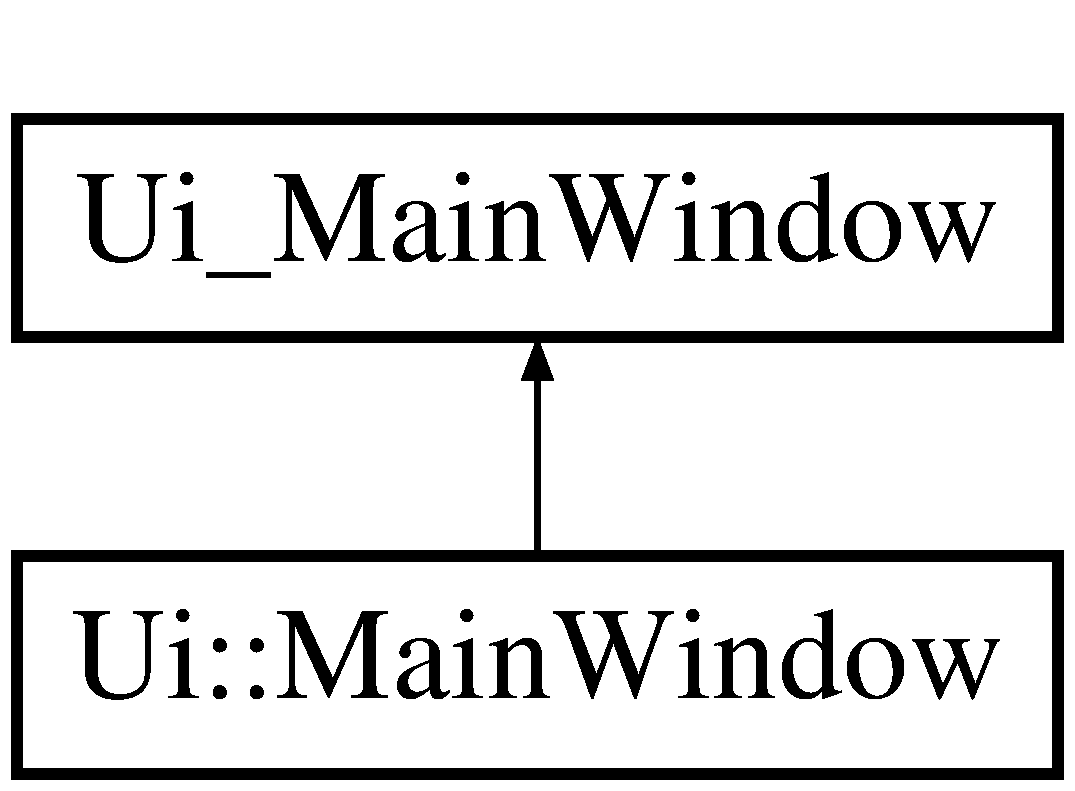
\includegraphics[height=2.000000cm]{class_ui___main_window}
\end{center}
\end{figure}
\subsection*{Public Member Functions}
\begin{DoxyCompactItemize}
\item 
\mbox{\Hypertarget{class_ui___main_window_acf4a0872c4c77d8f43a2ec66ed849b58}\label{class_ui___main_window_acf4a0872c4c77d8f43a2ec66ed849b58}} 
void {\bfseries setup\+Ui} (Q\+Main\+Window $\ast$\hyperlink{class_main_window}{Main\+Window})
\item 
\mbox{\Hypertarget{class_ui___main_window_a097dd160c3534a204904cb374412c618}\label{class_ui___main_window_a097dd160c3534a204904cb374412c618}} 
void {\bfseries retranslate\+Ui} (Q\+Main\+Window $\ast$\hyperlink{class_main_window}{Main\+Window})
\end{DoxyCompactItemize}
\subsection*{Public Attributes}
\begin{DoxyCompactItemize}
\item 
\mbox{\Hypertarget{class_ui___main_window_a30075506c2116c3ed4ff25e07ae75f81}\label{class_ui___main_window_a30075506c2116c3ed4ff25e07ae75f81}} 
Q\+Widget $\ast$ {\bfseries central\+Widget}
\item 
\mbox{\Hypertarget{class_ui___main_window_ad86caa6ccde1d44e62aef305d7dab7e2}\label{class_ui___main_window_ad86caa6ccde1d44e62aef305d7dab7e2}} 
Q\+Push\+Button $\ast$ {\bfseries cmd\+\_\+\+Ini\+Prueba}
\item 
\mbox{\Hypertarget{class_ui___main_window_ab676f235c393f334b7c07935d4007925}\label{class_ui___main_window_ab676f235c393f334b7c07935d4007925}} 
Q\+Widget $\ast$ {\bfseries widget}
\item 
\mbox{\Hypertarget{class_ui___main_window_aecd96a04789fcfec3f98d80390ad8184}\label{class_ui___main_window_aecd96a04789fcfec3f98d80390ad8184}} 
Q\+V\+Box\+Layout $\ast$ {\bfseries vertical\+Layout}
\item 
\mbox{\Hypertarget{class_ui___main_window_acd6fdc9ebacc4b25b834162380d75ce8}\label{class_ui___main_window_acd6fdc9ebacc4b25b834162380d75ce8}} 
Q\+H\+Box\+Layout $\ast$ {\bfseries horizontal\+Layout}
\item 
\mbox{\Hypertarget{class_ui___main_window_ad9c89133780f28e6efa2ec17ceb9cff5}\label{class_ui___main_window_ad9c89133780f28e6efa2ec17ceb9cff5}} 
Q\+Label $\ast$ {\bfseries label}
\item 
\mbox{\Hypertarget{class_ui___main_window_a471650c93c06a73d8ff60ed3eaecc247}\label{class_ui___main_window_a471650c93c06a73d8ff60ed3eaecc247}} 
Q\+Line\+Edit $\ast$ {\bfseries \+\_\+usrmainwindow}
\item 
\mbox{\Hypertarget{class_ui___main_window_a80867018070156432923d0266cc9fe25}\label{class_ui___main_window_a80867018070156432923d0266cc9fe25}} 
Q\+H\+Box\+Layout $\ast$ {\bfseries horizontal\+Layout\+\_\+2}
\item 
\mbox{\Hypertarget{class_ui___main_window_a2e2516d755e4dd53fc905dabddf2738a}\label{class_ui___main_window_a2e2516d755e4dd53fc905dabddf2738a}} 
Q\+Label $\ast$ {\bfseries label\+\_\+2}
\item 
\mbox{\Hypertarget{class_ui___main_window_aa65d0938fd3df4cf544fb82c90fbb1a4}\label{class_ui___main_window_aa65d0938fd3df4cf544fb82c90fbb1a4}} 
Q\+Line\+Edit $\ast$ {\bfseries \+\_\+usrmainwindow\+\_\+2}
\item 
\mbox{\Hypertarget{class_ui___main_window_a2be1c24ec9adfca18e1dcc951931457f}\label{class_ui___main_window_a2be1c24ec9adfca18e1dcc951931457f}} 
Q\+Menu\+Bar $\ast$ {\bfseries menu\+Bar}
\item 
\mbox{\Hypertarget{class_ui___main_window_a5172877001c8c7b4e0f6de50421867d1}\label{class_ui___main_window_a5172877001c8c7b4e0f6de50421867d1}} 
Q\+Tool\+Bar $\ast$ {\bfseries main\+Tool\+Bar}
\item 
\mbox{\Hypertarget{class_ui___main_window_a50fa481337604bcc8bf68de18ab16ecd}\label{class_ui___main_window_a50fa481337604bcc8bf68de18ab16ecd}} 
Q\+Status\+Bar $\ast$ {\bfseries status\+Bar}
\end{DoxyCompactItemize}


The documentation for this class was generated from the following file\+:\begin{DoxyCompactItemize}
\item 
/home/alseuser/\+Proyecto\+A\+L\+S\+E/build-\/\+Proyecto\+A\+L\+S\+E-\/\+Desktop-\/\+Debug/ui\+\_\+mainwindow.\+h\end{DoxyCompactItemize}

\hypertarget{class_ui__usuario}{}\section{Ui\+\_\+usuario Class Reference}
\label{class_ui__usuario}\index{Ui\+\_\+usuario@{Ui\+\_\+usuario}}
Inheritance diagram for Ui\+\_\+usuario\+:\begin{figure}[H]
\begin{center}
\leavevmode
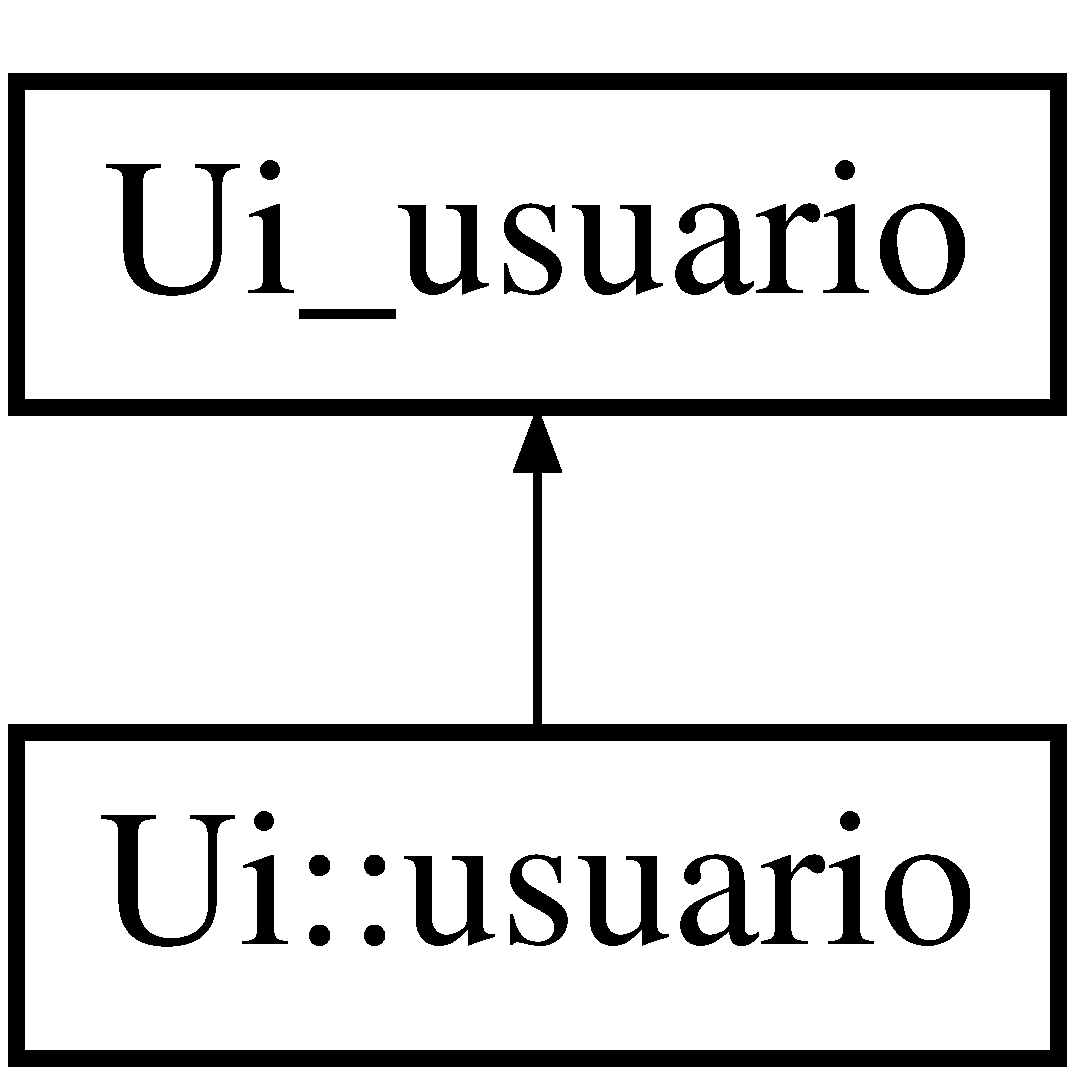
\includegraphics[height=2.000000cm]{class_ui__usuario}
\end{center}
\end{figure}
\subsection*{Public Member Functions}
\begin{DoxyCompactItemize}
\item 
\mbox{\Hypertarget{class_ui__usuario_a48c30dd275c61494b7892a0f1e95d675}\label{class_ui__usuario_a48c30dd275c61494b7892a0f1e95d675}} 
void {\bfseries setup\+Ui} (Q\+Dialog $\ast$\hyperlink{classusuario}{usuario})
\item 
\mbox{\Hypertarget{class_ui__usuario_a483718ca4dcb29af2e969a76ca3afee4}\label{class_ui__usuario_a483718ca4dcb29af2e969a76ca3afee4}} 
void {\bfseries retranslate\+Ui} (Q\+Dialog $\ast$\hyperlink{classusuario}{usuario})
\end{DoxyCompactItemize}
\subsection*{Public Attributes}
\begin{DoxyCompactItemize}
\item 
\mbox{\Hypertarget{class_ui__usuario_aaf194171c918371961f992de2c00f86f}\label{class_ui__usuario_aaf194171c918371961f992de2c00f86f}} 
Q\+Widget $\ast$ {\bfseries layout\+Widget}
\item 
\mbox{\Hypertarget{class_ui__usuario_a2eed23f73e18d74b1c9a781b93403e8f}\label{class_ui__usuario_a2eed23f73e18d74b1c9a781b93403e8f}} 
Q\+V\+Box\+Layout $\ast$ {\bfseries vertical\+Layout}
\item 
\mbox{\Hypertarget{class_ui__usuario_a397af6bf8d0d140334c5f2641aa63e59}\label{class_ui__usuario_a397af6bf8d0d140334c5f2641aa63e59}} 
Q\+Grid\+Layout $\ast$ {\bfseries grid\+Layout}
\item 
\mbox{\Hypertarget{class_ui__usuario_a5232eaa606361b4df1c8e9874904b3b1}\label{class_ui__usuario_a5232eaa606361b4df1c8e9874904b3b1}} 
Q\+Label $\ast$ {\bfseries label\+\_\+2}
\item 
\mbox{\Hypertarget{class_ui__usuario_ac8f8012f34f4cc089405da2f42e0a735}\label{class_ui__usuario_ac8f8012f34f4cc089405da2f42e0a735}} 
Q\+Line\+Edit $\ast$ {\bfseries \+\_\+username}
\item 
\mbox{\Hypertarget{class_ui__usuario_a24cc578c58c69b4d87e47987ce987d93}\label{class_ui__usuario_a24cc578c58c69b4d87e47987ce987d93}} 
Q\+Label $\ast$ {\bfseries label}
\item 
\mbox{\Hypertarget{class_ui__usuario_a2ea3093be83b06be3870eb62e44cee9c}\label{class_ui__usuario_a2ea3093be83b06be3870eb62e44cee9c}} 
Q\+Line\+Edit $\ast$ {\bfseries \+\_\+usrpassword}
\item 
\mbox{\Hypertarget{class_ui__usuario_a09cb4e0570b5329c0554b076214b50d8}\label{class_ui__usuario_a09cb4e0570b5329c0554b076214b50d8}} 
Q\+Dialog\+Button\+Box $\ast$ {\bfseries button\+Box}
\end{DoxyCompactItemize}


The documentation for this class was generated from the following file\+:\begin{DoxyCompactItemize}
\item 
/home/alseuser/\+Proyecto\+A\+L\+S\+E/build-\/\+Proyecto\+A\+L\+S\+E-\/\+Desktop-\/\+Debug/ui\+\_\+usuario.\+h\end{DoxyCompactItemize}

\hypertarget{structuser__data}{}\section{user\+\_\+data Struct Reference}
\label{structuser__data}\index{user\+\_\+data@{user\+\_\+data}}
\subsection*{Public Attributes}
\begin{DoxyCompactItemize}
\item 
\mbox{\Hypertarget{structuser__data_aacb4d4adab0081206fb60e06ae6ce0f0}\label{structuser__data_aacb4d4adab0081206fb60e06ae6ce0f0}} 
string {\bfseries nombre}
\item 
\mbox{\Hypertarget{structuser__data_a2c96e3aebe0fb4cc1ce25bf4de404924}\label{structuser__data_a2c96e3aebe0fb4cc1ce25bf4de404924}} 
string {\bfseries apellido}
\item 
\mbox{\Hypertarget{structuser__data_a200b6c316439f7cb74788cb953a4d8bd}\label{structuser__data_a200b6c316439f7cb74788cb953a4d8bd}} 
int {\bfseries doc\+\_\+id}
\item 
\mbox{\Hypertarget{structuser__data_ae4e769d36f8db851b28de099dd887fdd}\label{structuser__data_ae4e769d36f8db851b28de099dd887fdd}} 
int {\bfseries dia\+\_\+n}
\item 
\mbox{\Hypertarget{structuser__data_a7bde41ebb95c5bd69d2986060db8d97e}\label{structuser__data_a7bde41ebb95c5bd69d2986060db8d97e}} 
int {\bfseries mes\+\_\+n}
\item 
\mbox{\Hypertarget{structuser__data_a892d15908af2f7ac45b2027ebfedf41c}\label{structuser__data_a892d15908af2f7ac45b2027ebfedf41c}} 
int {\bfseries a\+\_\+n}
\end{DoxyCompactItemize}


The documentation for this struct was generated from the following file\+:\begin{DoxyCompactItemize}
\item 
/home/alseuser/\+Proyecto\+A\+L\+S\+E/datos\+\_\+usuario.\+h\end{DoxyCompactItemize}

\hypertarget{class_ui_1_1usuario}{}\section{Ui\+:\+:usuario Class Reference}
\label{class_ui_1_1usuario}\index{Ui\+::usuario@{Ui\+::usuario}}
Inheritance diagram for Ui\+:\+:usuario\+:\begin{figure}[H]
\begin{center}
\leavevmode
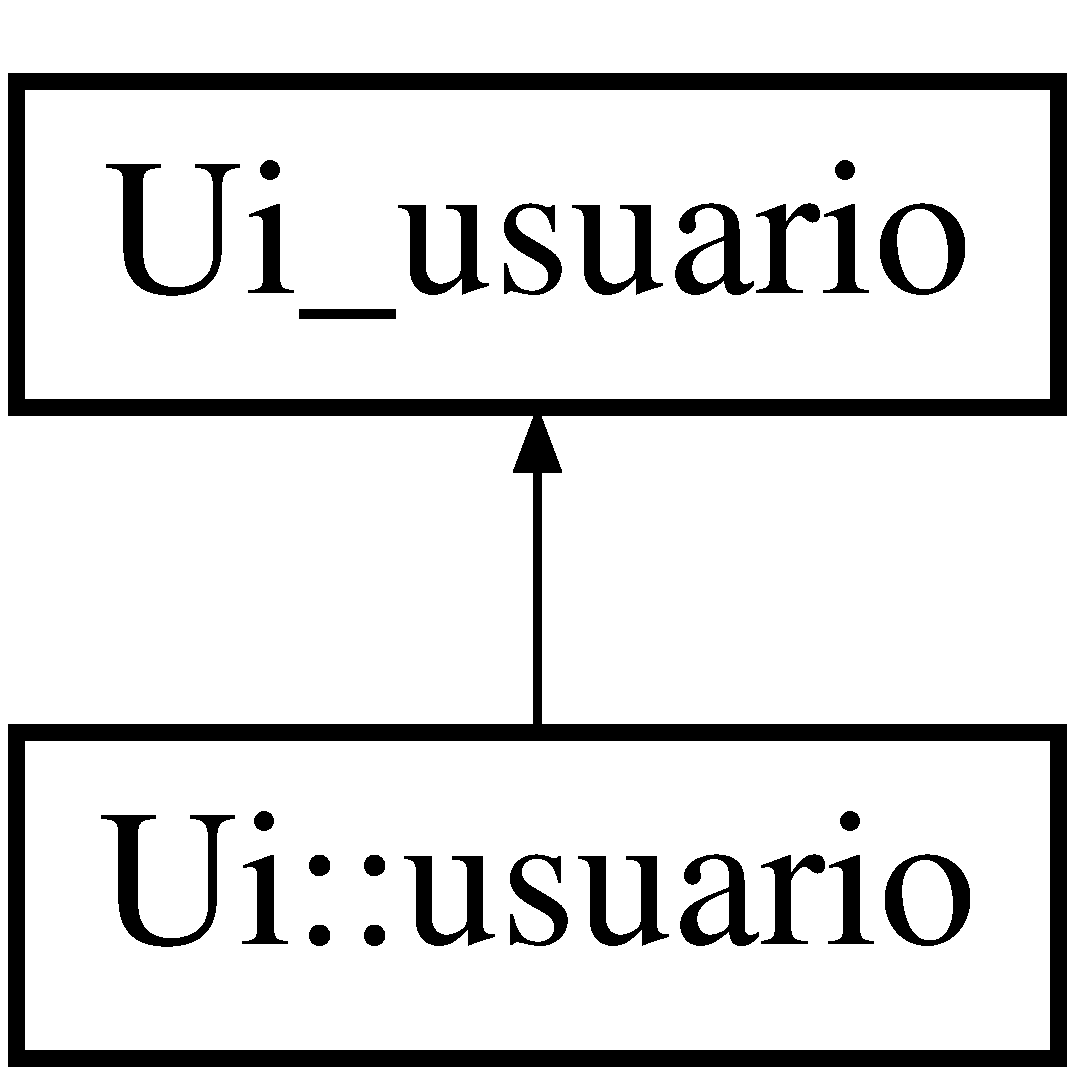
\includegraphics[height=2.000000cm]{class_ui_1_1usuario}
\end{center}
\end{figure}
\subsection*{Additional Inherited Members}


The documentation for this class was generated from the following file\+:\begin{DoxyCompactItemize}
\item 
/home/alseuser/\+Proyecto\+A\+L\+S\+E/build-\/\+Proyecto\+A\+L\+S\+E-\/\+Desktop-\/\+Debug/ui\+\_\+usuario.\+h\end{DoxyCompactItemize}

\hypertarget{classusuario}{}\section{usuario Class Reference}
\label{classusuario}\index{usuario@{usuario}}
Inheritance diagram for usuario\+:\begin{figure}[H]
\begin{center}
\leavevmode
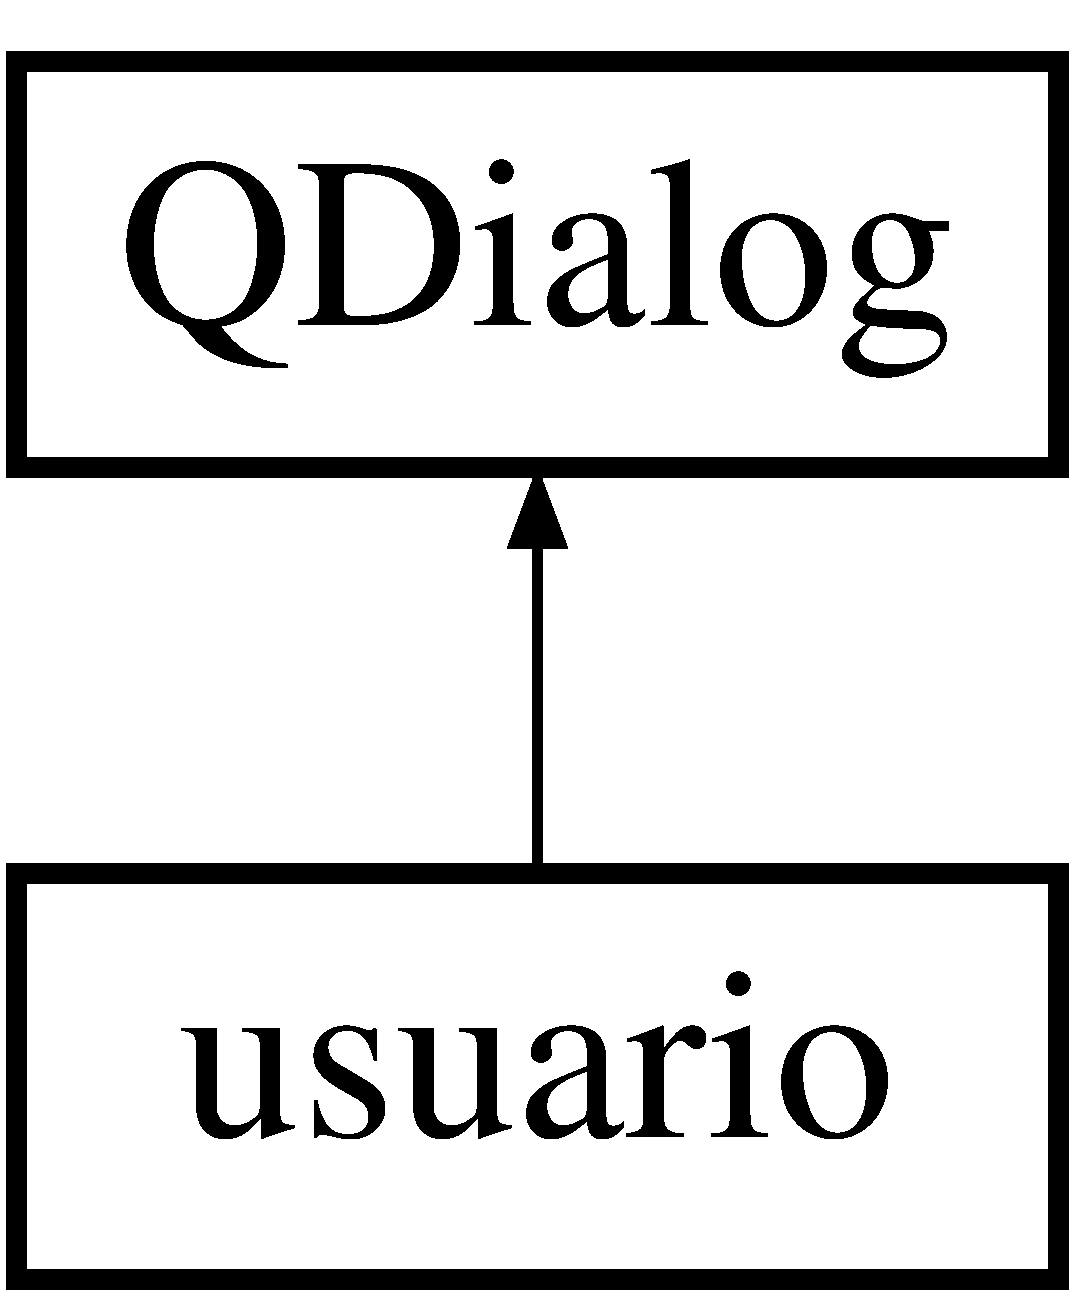
\includegraphics[height=2.000000cm]{classusuario}
\end{center}
\end{figure}
\subsection*{Public Member Functions}
\begin{DoxyCompactItemize}
\item 
\mbox{\Hypertarget{classusuario_a34821186e90424c9105221fb931e9ca0}\label{classusuario_a34821186e90424c9105221fb931e9ca0}} 
{\bfseries usuario} (Q\+Widget $\ast$parent=0)
\end{DoxyCompactItemize}


The documentation for this class was generated from the following files\+:\begin{DoxyCompactItemize}
\item 
/home/alseuser/\+Proyecto\+A\+L\+S\+E/usuario.\+h\item 
/home/alseuser/\+Proyecto\+A\+L\+S\+E/usuario.\+cpp\end{DoxyCompactItemize}

%--- End generated contents ---

% Index
\backmatter
\newpage
\phantomsection
\clearemptydoublepage
\addcontentsline{toc}{chapter}{Index}
\printindex

\end{document}
